\chapter{Beschreibung des Versuchsaufbaus und Durchführung des Experiments}

\section{Beschreibung des Versuchsaufbaus}
\label{sec:Beschreibung des Versuchsaufbaus}
Der Experimentelle Aufbau besteht im wesentlichen aus drei Hauptbestandteilen.
Dem Laser (grün) mit einer Wellenlänge von \SI{552}{\nano\meter}, der Festkörperprobe aus zusammengesetzen
Materialien und einen Spektrometer.
Im folgen werden die einzelnen verwendeten Bauteile in ihrem Verwendungszweck beschrieben.
In Abbildung ~\ref{fig:aufbau} ist der schematische Versuchsaufbau dargestellt.
\begin{figure}
    \centering
    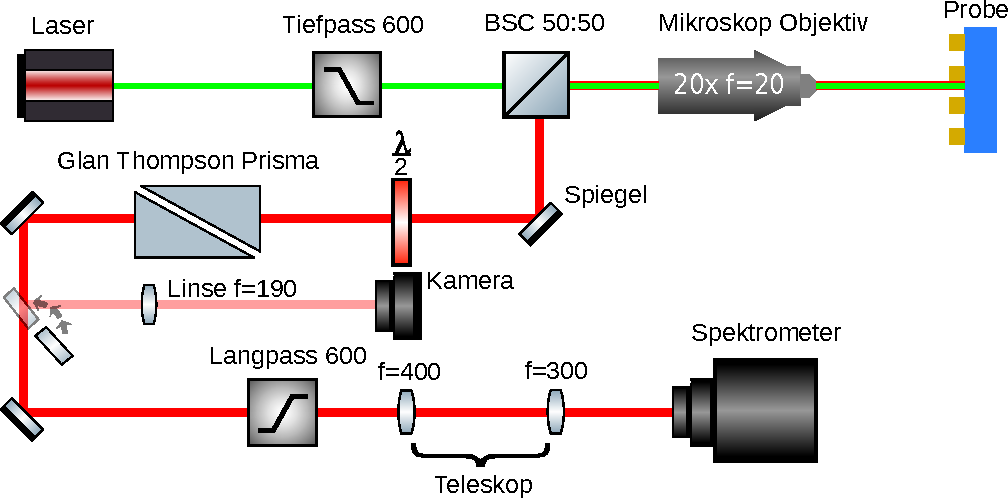
\includegraphics[scale=0.75]{./Plots/setup.pdf}
    \caption{Schematischer Versuchsaufbau mit allen effektiv wichtigen Versuchsbestandteilen.}
    \label{fig:aufbau}
\end{figure}
\FloatBarrier

Grundbestandteil des Versuchsaufbaus ist ein Dauerstrich-Diodenlaser der eine oben genannte Wellenlänge von 
\SI{552}{\nano\meter} liefert. 
Der Laserstrahl wird zu Beginn durch einen Tiefpass geschickt, mit einer Grenzwellenlänge von 
\SI{600}{\nano\meter}. Der Tiefpass sorgt dafür das nur Wellenlängen durchgelassen werden die 
kleiner als die angegebene Wellenlänge ist. Auf den ersten Blick scheint dies überflüssig, da der
verwendete Laser sowieso nur eine kleinere Wellenlänge liefert, doch um Störeffekte des Lasers 
konkret, dass Aussenden von Wellenlängen im Bereich des späteren Effekts ist zur Sicherheit ein
Tiefpass installiert worden. 
Nach dem Tiefpass gelangt der Laserstrahl in einen 
nicht polarisierenden Strahlteilerwürfel (kurz BSC).\footnote{BSC (englisch) Beam-splitter-cube.}
Der verwendete BSC hat im Inneren eine Grenzfläche, die unter 45° zu den Seiten 
steht und $\SI{50}{\percent}$ der Lichtintensität transmittiert und $\SI{50}{\percent}$ reflektiert.
Das bedeutet konkret, dass 
\SI{50}{\percent} der Intensität weiter gerade aus laufen und anschließend auf das Mikroskopobjektiv 
treffen können. Im Mikroskopobjektiv welches eine numerische Apertur von 0,4 besitzt, wird 
das Laserlicht auf die Probe fokussiert. Durch die numerische Apertur kann ein
halber objektseitiger Öffnungswinkel von $\theta \approx \SI{24}{\degree}$ realisiert werden. 
Dieser ist später ausschlaggebend für Ven detektierbaren Winkelbereich der von der Probe emittierten
Intensität. 
Die zu untersuchende Festkörperprobe unterliegt ständiger Kühlung mit flüssigem Helium und befindet
sich in einem  Durchfluss-Kryostaten. Die Probentemperatur kann zudem extern reguliert werden, welches
über  ein elektrisches Heizelement geschieht.
Dabei gibt es zu beachten, dass sich der Temperatursensor nicht unmittelbar auf der 
Probenoberfläche befindet, sondern in einem isolierten Tubus ein Stück weiter von der Probe entfernt
ist. Eine direkte Installation auf der Probe ist technisch nicht möglich. 
Links und rechts neben der Probe befinden sich zwei Spulen, die maximal eine Flussdichte von
\SI{0.5}{\tesla} erzeugen können. 
Die Spulen sind an eine externe Wasserkühlung angeschlossen und können je nach Bedarf 
über Computersoftware angesteuert werden um die gewünschte Flussdichte zu erzeugen. 
Nachdem das Laserlicht auf die Probe gefallen ist, emittiert die Probe Photolumineszenzlicht (PL).
Das emittierte PL wird von der Festkörperprobe in alle Richtungen diffus abgegeben und 
wird von dem Mikroskopobjektiv in einem Winkelbereich von $\pm \SI{24}{\degree}$ aufgesammelt. 
Danach läuft es auf dem selben Weg rückwerts wie zuvor das Laserlicht bis zu der Stelle des BSC.
Am BSC wird das PL dann in rechten Winkel reflektiert (vgl. Abbildung ~\ref{fig:aufbau}) und umgelenkt sodass sie 
auf ein $\sfrac{\lambda}{2}$-Plättchen trifft.
Das $\sfrac{\lambda}{2}$-Plättchen wird hier nur der Vollständigkeit aufgeführt, in dem Experiment
wird es so ausgerichtet das es keinen Effekt hat. 
Bei anderer Ausrichtung liese sich überprüfen ob die Messung auch für s-polarisiertes PL
funktioniert.
Effektiv trifft das Licht welches verschiedene Polarisationen hat auf das Glan-Thomson-Prisma.
Das Glan wirkt hierbei wie ein Filter der dafür sorgt das nur p-polarisiertes Licht hindurch kann.
Das ist wichtig denn der zu messende Effekt tritt nur bei genannter Polarisation auf.
Wird das Glan weggelassen, so bleiben die unterschiedlichen Polarisationen erhalten
und es würde nur weniger Effekt messbar sein. 
Nachdem das PL das Glan-Thomson-Prisma passiert hat, wird es vor Beginn einer jeden Messung zuerst
mit Hilfe eines Klappspiegels und einer Linse auf eine Kamera fokussiert. 
Die Abbildung auf die Kamera erfolgt um sicherzugehen, dass die Probe sich im Fokus des 
Mikroskopobjektivs befindet.
Anschließend wird der Klappspiegel zugeklappt und das PL gelangt nach weiterer Umlenkung in einen 
Langpass mit einer Grenzwellenlänge von \SI{600}{\nano\meter}. 
Der Langpass sorgt dafür, dass kein Laserlicht oder andere Fremdstrahlung
welche bis zu diesem Punkt gelangt ist weiter propagieren kann. 
Da das Maximum des PL bei $\approx \SI{740}{\nano\meter}$ liegt, 
kann dieses den Langpass ungehindert durchdringen.
Anschließend gelangt das PL in eine Kombination aus zwei Linsen mit unterschiedlichen Brennweiten.
Diese wirken zusammen wie ein Teleskop, welches in der Lage ist die Direktionalität des Effekts 
im Spektrometer darzustellen.
\footnote{Das Mikroskopobjektiv bildet die Winkelinformation in eine Fourierebene ab,
welche durch das Teleskop real im Spektrometersicht darstellbar ist.} 
Im Spektrometer angekommen wird das Licht durch den Monochromator nach Wellenlänge separiert und 
anschließend durch die CCD (charge-coupled device) registriert.

\section{Durchführung des Experiments}
Bevor mit einer Messung begonnen werden kann muss die Probe in den Fokus des Mikroskopobjektivs 
gebracht werden. 
Mit einem Klappspiegel und einer zusätzlichen Linse wird eine Abbildung des 
Fokuspunktes auf der Kamera erzeugt. 
Die Probe kann nun über Mikrometerschrauben, welche sich an der 
Probenhalterung befinden justiert werden.
Das Bild welches die Kamera aufnimmt wird Digital auf einen Computerbildschirm dargestellt. 
Ist die Fokussierung abgeschlossen kann der Spiegel entfernt werden und mit der eigentlichen Messung 
wird begonnen.
Alle Messungen werden mit Hilfe entsprechende Computersoftware gestartet.
%evtl im anderen kapitel übr die probe
%Der Probenname ist 022818A 250nm. 
%Wobei sich die Angabe 250nm auf die $\SI{250}{\nano\meter}$ Abstände des Goldgitters beziehen.
%Das Experiment findet insgesamt für acht unterschiedliche Temperaturen statt.
%
%ALSO DAS LIEBER RAUSSLASSEN?
%Die unterschiedlichen Messreihen werden nicht alle an dem selben Tag aufgenommen, sondern sind
%im Zeitraum von 14. Juli 2020 bis zum 31. Juli 2020 entstanden.
%Dies ist unter anderem um die Reproduzierbarkeit von Messergebnisses sicherzustellen geschehen.
Zu Beginn der Messung wird die Temperatur so eingestellt, dass der Temperatursensor \SI{4}{\kelvin} zeigt. 
Danach erfolgt die Messung des Hintergrunds.
Der Hintergrund setzt sich unter anderem aus dem einfallendem Umgebungslicht und 
dem Dunkelstromausschlags (Rauschen der CCD) zusammen, welcher trotz Kühlung vorhanden ist.
Im nächsten Schritt wird die gewünschte Temperatur über das Heizelement und durch 
Kontrolle des Heliumflusses eingestellt. 
Es werden abwechselnd Spektren bei positivem und negativem Magnetfeld aufgenommen. 
Jedes Spektrum besteht aus 16 Einzelbildern mit jeweils 3 Sekunden Belichtungszeit, die aufaddiert werden.
Die Einzelbilder werden gemacht, damit die CCD welche die Intensität erfasst nicht zum sättigen 
gebracht wird, was zur Folge hätte das keine oder kleine Unterschiede nicht mehr messbar sind.
Der Wechsel zwischen positiver und negativer Flussdichte wird 26 Mal wiederholt, damit 
wird versucht Störeffekten, (z.B. Änderungen der Laserintensität) die sich erst über 
längere Messdauer einstellen könnten, entgegenzuwirken.
Nach jeder Messung wird die Temperatur auf die jeweils nächst zu messende Temperatur angeglichen
und mit der nächsten Messung wird begonnen.
Die Messdaten werden in Textdokumenten gespeichert, die die um den Hintergrund 
reduzierten Intensitäten beinhalten.